\documentclass[10pt,a4paper]{article}
\usepackage[T1]{fontenc}
\usepackage[scaled]{helvet}
\usepackage{cite}
\usepackage{url}
\usepackage{graphicx}
\usepackage{listings}
\usepackage{float}
\usepackage{amsmath}
\usepackage{listings}
\usepackage{color}
 
\definecolor{dkgreen}{rgb}{0,0.6,0}
\definecolor{gray}{rgb}{0.5,0.5,0.5}
\definecolor{mauve}{rgb}{0.58,0,0.82}
\lstset{ %
  language=Octave,                % the language of the code
  basicstyle=\footnotesize,           % the size of the fonts that are used for the code
  numbers=left,                   % where to put the line-numbers
  numberstyle=\tiny\color{gray},  % the style that is used for the line-numbers
  stepnumber=1,                   % the step between two line-numbers. If it's 1, each line 
                                  % will be numbered
  numbersep=5pt,                  % how far the line-numbers are from the code
  backgroundcolor=\color{white},      % choose the background color. You must add \usepackage{color}
  showspaces=false,               % show spaces adding particular underscores
  showstringspaces=true,         % underline spaces within strings
  showtabs=false,                 % show tabs within strings adding particular underscores
  frame=none,                   % adds a frame around the code
  rulecolor=\color{black},        % if not set, the frame-color may be changed on line-breaks within not-black text (e.g. commens (green here))
  tabsize=2,                      % sets default tabsize to 2 spaces
  breaklines=true,                % sets automatic line breaking
  breakatwhitespace=false,        % sets if automatic breaks should only happen at whitespace
  keywordstyle=\color{blue},          % keyword style
  commentstyle=\color{dkgreen},       % comment style
  stringstyle=\color{mauve},         % string literal style
  escapeinside={\%*}{*)},            % if you want to add LaTeX within your code
  morekeywords={*,...}               % if you want to add more keywords to the set
}
\usepackage{amssymb}
\usepackage{fancyhdr}
\usepackage{lastpage}
\floatstyle{boxed} 
\restylefloat{figure}
\renewcommand*\familydefault{\sfdefault}
\title{Management of Main Memory}
\author{David Lynch - david.lynch@raglansoftware.com }
\begin{document}
\maketitle
\begin{abstract}
The final topic in the Operating Systems section of this course deals with the management of main memory. Once you are comfortable with creating processes, understanding how processes communicate with each other and taking advantage of threads the next concern lies with understanding management of one of the systems most vital resource. As a programmer, the importance of this understanding will become clear as soon as you start writing any non-trivial applications, particularly in the enterprise space. How the operating system manages memory allocated to your process has an effect on everything from how your program functions to the performance of your application. 
\end{abstract}
\section{Main Memory}
Processes are assigned an address space defined by a {\bf base register} and a {\bf limit register}. Hardware and the operating system provide protections around user processes accessing the addresses of other processes or any locations in kernel memory. However, operations that execute in kernel mode may have access to the full address space. 
\newline\newline
A process can be located anywhere in memory, and its starting location, together with other significant locations are bound to re-locatable addresses. This address in turn is part of a mapping between {\bf logical} and {\bf physical} address locations. Binding to address locations can happen at {\bf compile time}, {\bf load time} and {\bf execution time}. In the first instance, address locations are pre-compiled to pre-determined locations in memory. With load time binding, the program can be re-located across the address space. During execution time a process may, for example, be moved from one segment in memory to another. This is determined by various characteristics of the application at runtime. 
\subsection{Logical vs. Physical Address Space}
Addresses generated by the CPU are referred to as {\bf logical addresses}. The address seen by the MMU, and stored in the {\bf memory address register} or MAR is referred to as the {\bf physical address}. The set of all logical addresses generated by a program is called it's {\bf virtual address space}. Conversely, the {\bf physical address space} is the set of all the physical addresses associated with the processes. The MMU is responsible for the mapping that exists between the two views. 
\subsection{Dynamic Loading}
So far we have required the entire process to exist in physical memory for it to be executable. Dynamic loading allows a routine to be left on secondary storage until it is required. This can be more memory-space efficient, but can have performance ramifications. For this to work, routines are kept on disk in a relocatable format. Before another routine is called the running routine may check if the new routine is already loaded. A loader then loads the routine into memory, adjusting the address space before handing control back to the program. No special operating systems intervention is required for this functionality. 
\subsection{Dynamic Linking and Shared Libraries}
Libraries that are not dynamically linked by a program are termed statically linked. Each process keeps its own copy of a statically linked library in memory. Dynamically linked libraries exist initially only as {\bf stubs} in memory. This stub contains instructions on how to link the library to the program. One of two courses of action are possible when a dynamically linked library is required. In the case where library has not been loaded from disk, it is loaded into memory. Otherwise, the stub will replace itself with a pointer to the address to which the dynamically linked library has been stored to memory. In this manner, multiple programs that use the same libraries will reference one copy of the code in memory. Dynamic Linking requires help from the OS if multiple processes are required to access the same address. 
\subsection{Swapping}
Processes must be in main memory to be executed, but at various points may be swapped from memory to the backing store. For example, when a process is suspended, the memory manager may move the no longer executing process from main memory to disk. Processes may be swapped back into a different address space at some point after they are swapped out. The CPU calls the {\bf dispatcher} which checks to see if the next process in the ready queue is in memory. If it is not in memory, the process gets loaded. During this action, other processes that are not under execution may be swapped out to free up sufficient memory for the replacement process. {\bf Context Switch} time is a pure cost in this process, and is a direct function of the size of the program being executed, the performance characteristics of the backing store and other underlying hardware. For a process to be a candidate for disk swapping it must be {\bf completely idle}. In particular, waiting on I/O or for the CPU is not a sufficient reason to swap the process to the disk. 
\subsection{Memory Allocation}
In order to manage memory, division into fixed size partitions is the simplest approach. Each of these partitions will contain exactly one process. With this strategy, the number of processes is bound by the size of the physical memory space. Each partition is known as a {\bf hole}. The process acquires and releases each hole as it is swapped in and out of memory. The operating system may merge smaller holes into bigger ones to facilitate the loading of bigger processes into memory. The problem of satisfying a request for $n$ bytes of space from a list of free memory holes is one of dynamic allocation. One approach is to allocate the first hole that is large enough. The {\bf best fit} approach will allocate the smallest hole that is big enough, leaving the smallest hole left over. Lastly, the {\bf worst fit} approach picks the worst possible fit for the process, ensuring the largest hole remains. {\bf First fit} is faster, but both best and worst fit have better, and similar memory utilization characteristics. 
\subsection{Fragmentation}
In any allocation strategy when small unusable memory segments are left over, the system is suffering from memory fragmentation. There are two flavours of fragmentation that essentially differ by whether the left over memory that is unusable is contained in an allocated block, or in free space external to a block. 
\subsubsection{External Fragmentation}
The previously discussed strategies will inevitably cause external fragmentation over the lifetime of a power-up. Swapping back and forth from disk using these strategies will cause small unusable holes of memory to appear. Statistical analysis of first fit shows that given $n$ holes of memory, another $0.5n$ holes will be lost to fragmentation. In order to combat this phenomenon, {\bf compaction} can be implemented. This is the shuffling of free memory so that smaller blocks become one block. One approach to compaction is to move processes to lower sections of memory and holes to higher sections of memory. However, compaction is pure cost and, depending on the characteristics of the system, is an expensive operation. We will talk about how the JVM uses compaction in the next article. 
\subsubsection{Internal Fragmentation}
Generally holes of memory will not be allocated in the exact size required. The overhead on minute leftover blocks can be worse than giving free memory away. However, this has the effect of leaving memory allocated to the process that is not actually used by that process, nor is it usable by any other process. 
\section{Paging}
Paging is a memory management scheme that allows the physical address space of a process to be non-contiguous. This avoids the problem of fitting memory chunks of various sizes into contiguous main memory. This is typically implemented in hardware with very low level OS support. Physical memory is broken into fixed sizes known as {\bf frames}. Logical memory is broken into blocks of the same size known as {\bf pages}. When a process is executing its pages are loaded into available frames. Every CPU generated address is divided into {\bf page number} and {\bf page offset}. The page number is an index into the {\bf page table}, which holds the direct logical-to-physical mapping. It contains the base address of each page and the address of the corresponding frame in physical memory. The size of the page is fixed and defined by the hardware, but can range from 512-bytes to 16 megabytes. 
\newline\newline
If the logical address size is $2^n$ and the page size is $2^m$ addressing units then the higher order $m-n$ bits are the page number $p$ and the lower order $n$ bits are the {\bf page offset} or {\bf displacement} denoted as $d$. Figures \ref{paging} and \ref{page mapping} show both the general configuration and an example mapping. 
\begin{figure}
\caption{The basics of paging.\cite{OSCONCEPTS}}
\begin{center}
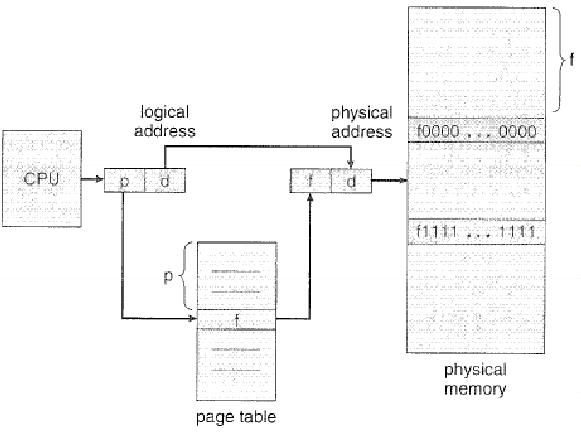
\includegraphics[scale=0.5]{../images/paging.png}
\label{paging}
\end{center}
\end{figure}
\begin{figure}
\caption{An example page mapping. \cite{OSCONCEPTS}}
\begin{center}
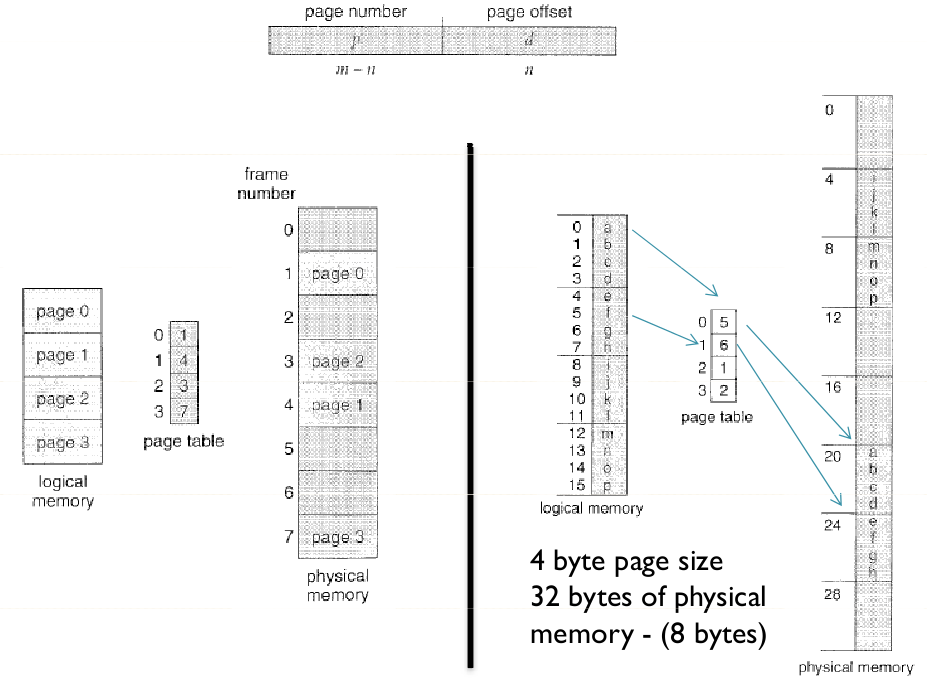
\includegraphics[scale=0.45]{../images/page-mapping.png}
\label{page mapping}
\end{center}
\end{figure}
Since any free frame can be allocated to a process that needs it, there is no external fragmentation. However, since frames are allocated in units, any time a process does not coincide with a page boundary we get internal fragmentation. For example, given a page-size of 2048 bytes, a process of size 72,766 bytes needs 35 full pages plus 1086 bytes left over. Therefore 36 pages are allocated and 962 bytes are lost to internal fragmentation. The statistical average expense is one have page of internal fragmentation per process. 
\newline\newline
A {\bf frame table} is managed by the OS which details frame availability and allocation. Each entry contains the state of the frame and to which page the frame is mapped. The OS will also manage one {\bf page table} per process, meaning paging will add to context switch overhead. 
\newline\newline 
A major advantage of paging is the sharing of common code. {\bf Re-entrant} code is non self-modifiying code that is pure code that can be share accross processes. Page sharing can also facilitate and support the {\bf shared memory} IPC concept. Most modern operating systems use hierarchical paging. With a address spaces of sizes $2^24$ the size of the page table can become prohibitively large. This is known as {\bf multi-level} paging. 
\subsubsection{Hardware Support}
The OS will allocate a page table per procesess, a pointer to which will be stored as part of the process control block. Hardware support is typically in the form of dedicated registers designed to make address translation efficent. Use of {\bf page-table base-registers} is feasible for page tables with small sizes. Essentially, this register contains a pointer to location 0 in the page table of the currently executing process. This value will be loaded from the PCB associated with the process that is currently executing. 
\newline\newline
However, for the above approach, we need at least two look ups into memory. Firstly, we need to acquire the page-table base register mapping and secondly we must load the page-table contents into memory. A {\bf translation look aside buffer} is an associative high speed cache used to alleviate look-ups into a page table associated with one or more processes. Figure \ref{page-tlb} illustrates how the TLB acts as as a cache in potentially removing the look-up into the page-table. Note particularly the difference between what happens when there is a cache hit vs. what happens when there is a cache miss.
\newline\newline
TLBs of this nature are expensive on-MMU caches, so they are typically limited to between 64 and 1024 entries maximum.
\begin{figure}
\caption{Paging assisted by a TLB.\cite{OSCONCEPTS}}
\begin{center}
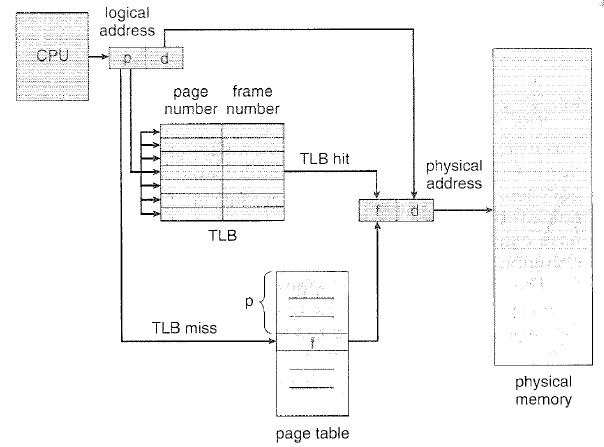
\includegraphics[scale=0.45]{../images/page-tlb.png}
\label{page-tlb}
\end{center}
\end{figure}
\section{Segmentation}
Segmentation is an alternative memory management scheme that supports the users view of memory by creating a logical address space as a collection of segments of various sizes. Each logical address has a {\bf segment number} and an {\bf offset}. For example, the C compiler creates seperate segments for code, global variables, heap, stacks and the standard C template library. A {\bf segment table} is used to map the one dimentional view of memory to the two dimensional concept of segments. Each segment has an {\bf segment base} and {\bf segment limit} pointer that demarcates the bounds of the segment in memory. Figure \ref{seg} shows in detail how segments relate to logical address space and how the segment table maps each segment to physical memory via offsets into the windows defined by the segment limit and base pointers.
\begin{figure}
\caption{Segments as they map to physical memory \cite{OSCONCEPTS}}
\begin{center}
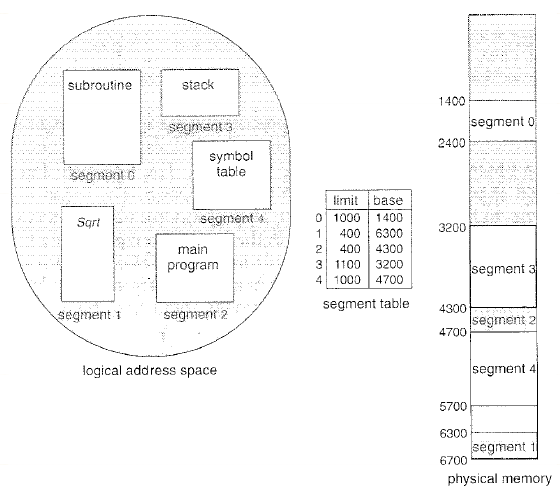
\includegraphics[scale=0.5]{../images/segmentation.png}
\label{seg}
\end{center}
\end{figure}
\section{Virtual Memory}
The memory management techniques discussed so far require the process to be entirely in memory. Virtual memory allows execution of a process that is not completely in main memory while it is executing. Programs often have code paths that are rarely executed and not often required in main memory. This includes rarely executed exception handling. When programming, the coder often over-provisions array lists and tables, meaning that with pure paging, unused pages of memory can be moved into memory unnecessarily. Even when a program is totally required, the is usually some window of time where all of the program need not be loaded to memory.
\newline\newline
There are numerous benefits to virtual memory. Firstly, a program can be much larger than physical memory. Moreover, programmers don't really need to worry too much if their programs are larger than physical memory, or if their arrays are over-provisioned. To some extent, the operating system will help out leaving the programmer to worry about other things. Secondly, virtual memory allows even more processes to run concurrently than pure paging or segmentation without virtual memory. Thirdly, and with the caveat that virtual memory is tuned correctly, it reduces in total the I/O of swapping a full process in and out of memory. Virtual memory is complex and difficult to implement and must be effectively managed by both the OS and the user of the system. 
\newline\newline
Virtual memory further re-enforces the concept of separation of logical memory as perceived by users from physical memory. The virtual address space now refers to the logical view of how a process is stored in memory. A breakdown of the virtual address spaces is illustrated in figure \ref{virtmemlog}. The {\bf heap} grows upwards in memory and is used for dynamic memory allocation. The {\bf stack} grows downwards in memory and facilitates successive function calls. There exists a hole between these two which is blank until the stack and or the heap grows into it. Virtual address spaces that include holes are known as sparse address spaces. Figure \ref{virtmem} shows how pages of virtual memory are mapped to physical memory, both main and backing store via a memory map.
\begin{figure}
\caption{Logical Virtual Memory \cite{OSCONCEPTS}}
\begin{center}
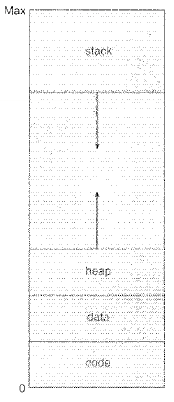
\includegraphics[scale=0.6]{../images/virtmem-log.png}
\label{virtmemlog}
\end{center}
\end{figure}
\begin{figure}
\caption{A virtual memory system \cite{OSCONCEPTS}}
\begin{center}
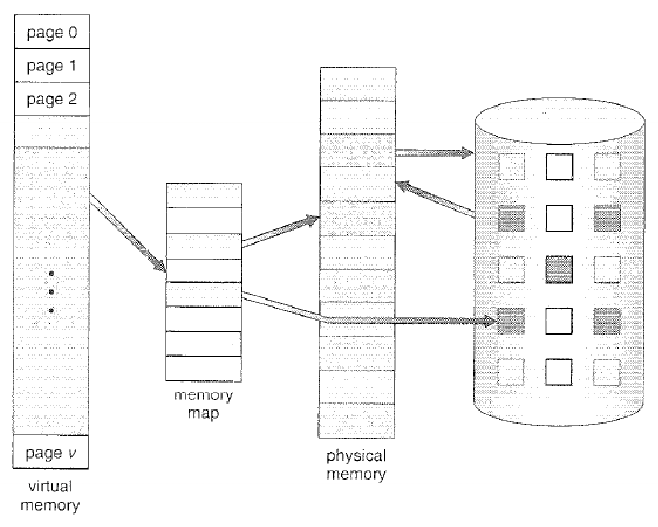
\includegraphics[scale=0.45]{../images/virtmem.png}
\label{virtmem}
\end{center}
\end{figure}
\subsection{Demand Paging}
With demand paging, pages are loaded into memory only as they are needed. Pages that are never accessed are never loaded into physical memory and remain on backing store. This is known as {\bf lazy swapping}. This is similar to a paging system with swapping where processes reside, at least at the page level, in secondary memory. A swapper is disticnt from a pager since a swapper is responsible for swapping entire processes to and from memory. A {\bf pager} is concerned with the swapping of individual pages out of the processes. Figure \ref{demandpaging} illustrates two processes as they exist in main memory, and hows how only segments of each code section are swapped in and out using the demand paging approach. 
\begin{figure}
\caption{Demand Paging \cite{OSCONCEPTS}}
\begin{center}
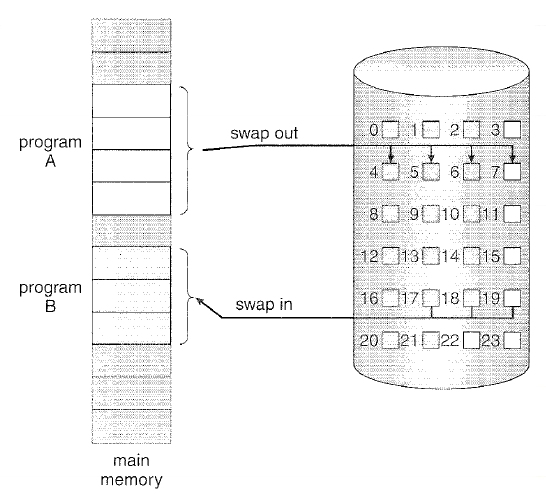
\includegraphics[scale=0.45]{../images/demand-paging.png}
\label{demandpaging}
\end{center}
\end{figure}
When a process is to be swapped in, the pager guesses which pages will be used before the process will be swapped out again and these pages are brought into memory. Similar to a cache a {\bf valid bit} can help distinguis between pages that are on the disk or in main memory.  Pages that are in memory are termed {\bf memory resident}. Access to a page that is not in memory causes a {\bf page fault trap} which must be handled. Figure \ref{demandex} shows a concrete example of values that map from logical memory to physical memory via the page table. 
\begin{figure}
\caption{Demand Paging Example \cite{OSCONCEPTS}}
\begin{center}
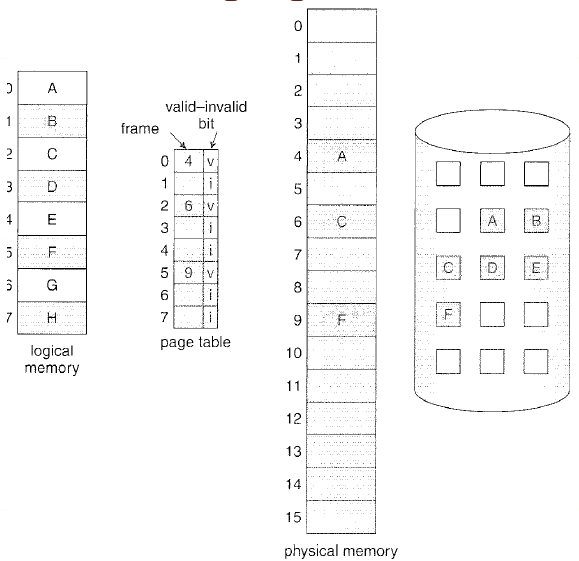
\includegraphics[scale=0.45]{../images/demand-paging-example.png}
\label{demandex}
\end{center}
\end{figure}
\subsubsection{Handling a Page Fault}
The page fault interrupt handler is concerned with a number of things. Firstly, the PCB internal table is checked to determine if the address is a valid one for the process in question. If the address is not in the calling processes address space then an error is generated and the process is killed. Otherwise, we need to move the requested page into memory. To do so, the pager needs to find a free frame. Next, it needs to schedule a disk read to read data into the frame. Next, the PCBs internal table and the page table is modified to indicate the page is now in memory. As with all interrupt handlers, the instruction that initiated the trap is restarted.
\begin{figure}
\caption{Handling a Page Fault \cite{OSCONCEPTS}}
\begin{center}
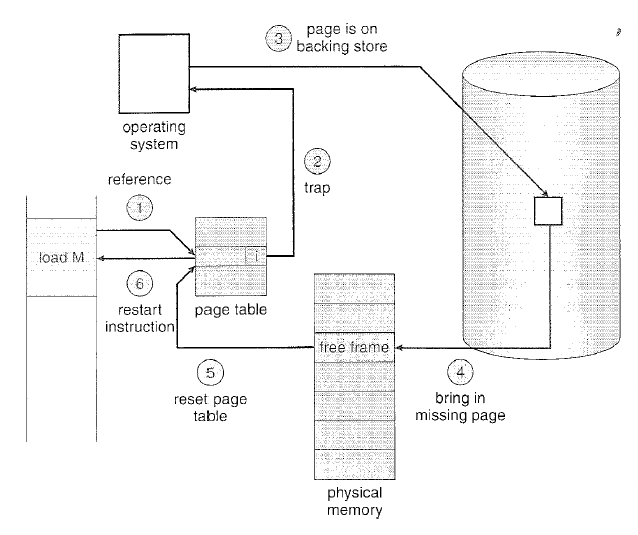
\includegraphics[scale=0.45]{../images/page-fault.png}
\label{page-fault}
\end{center}
\end{figure}
It is possible, though possibly not desirable, to start a process with zero pages in memory. This causes immediate faulting upon execution and is known as {\bf pure demand paging}. Since page faulting is pure overhead, it is desirable to minimize time spent swapping. When we consider the principle of locality of reference, however, the worst case scenario of one page fault per instruction is extremely unlikely. Nevertheless, there are still optimizations that can be gained by tuning various parameters around demand paging.
\subsubsection{Performance}
Due to the expense of interacting with backing store, demand paging has the potential to have a significant impact on the overall performance of a computer system. The {\bf effective access time} for demand paged memory is our most interesting measure when considering performance. As long as there are no faults the EAT is equal to the memory access time. If there is a fault, it must be handled via several steps. Our effective access time can be capture by the following expression.
\begin{equation}
\begin{split}
&T_{effective} = (1 - P_{fault}) * T_{access} + P_{fault} * T_{fault}\\
\end{split}
\end{equation}
\newline\newline
\begin{figure}
\caption{Steps in completing a page fault}
\begin{center}
\begin{tabular}{| l | l | }
  \hline
  Trap to Operating System. \\
  Save Registers and Process State. \\
  Determine if interrupt was a page fault. \\
  Check the legality of the reference. \\
  Determine the location of the page on disk. \\
  Read from the disk to the free frame. Includes I/O wait. \\
  While waiting allocate the CPU something else. \\
  Receive an interrupt indicating disk I/O is finished.  \\
  Switch out other processes from the CPU. \\
  Correct the page table showing the desired page is in memory. \\
  Wait again for the CPU. \\  
  Restore state from the PCB and resume interrupted instruction. \\
  \hline
\end{tabular}
\label{pfsteps}
\end{center}
\end{figure}
Figure \ref{pfsteps} shows a list of things to be considered when handling a page fault. To service a page fault interrupt one to several hundred instructions of 1 to 100 microseconds is required. To read in the page from disk reads of the order of 8 milliseconds are not uncommon. A typical memory access cycle will complete in the order of microseconds. Restarting the process is also measured in orders of tens of microseconds.   



\bibliography{../biblio/techfundamentals.bib}{}
\bibliographystyle{plain}
\begin{center}
{\small \copyright  David Lynch 2012. Do not reproduce without written permission.}
\end{center}
\end{document}
